\documentclass[10pt,a4paper,hidelinks]{article}
\usepackage[utf8]{inputenc}
\usepackage[english]{babel}
\usepackage[T1]{fontenc}

\newcommand{\documentStatus}{DRAFT}


\usepackage{amsmath}
\usepackage{amsfonts}
\usepackage{amssymb}
\usepackage{graphicx}
\usepackage{lmodern}
\usepackage{tikz}
\usetikzlibrary{positioning}
\usepackage{epigraph} 
\usepackage[left=2.5cm,
            right=2.5cm,
            top=2cm,
            bottom=2cm]{geometry}
\usepackage{setspace}
\usepackage{caption}
\usepackage{subcaption}
\usepackage{epigraph}
\usepackage{pdflscape}
\usepackage{pgfplots}

\usepackage{titlesec}
\usepackage{tcolorbox}
\usepackage{background}
\usepackage{url}
\usepackage[pdfauthor={Pierre Jézégou},
            pdftitle={ADS assignement},
            pdfsubject={Word games},
            pdfkeywords={}]{hyperref}
\usepackage{wrapfig}


\backgroundsetup{contents=\documentStatus, color=\watermarkColor}

\usepackage{fancyhdr}
\usepackage{textpos}
\usepackage{sectsty}
\usepackage{xcolor}

\setlength{\parindent}{0pt}

%%%%%%%%%%%%%%% Colors %%%%%%%%%%%%%%%
\subsectionfont{\color{fib_red}}
\subsubsectionfont{\color{fib_red}}
\renewcommand\fbox{\fcolorbox{black}{fib_red!20}}

\definecolor{fib_red}{RGB}{191,21,64}
\definecolor{fib_gray}{RGB}{111,111,111}
\definecolor{blue_upc}{RGB}{52,120,186}

\usepackage{listings}
\lstdefinestyle{mystyle}{
  backgroundcolor=\color{gray!10},
  stringstyle=\color{green!60!black!80},
  keywordstyle=\color{fib_red},
  numberstyle=\tiny\color{fib_gray},
  commentstyle=\color{blue_upc},
  basicstyle=\ttfamily\footnotesize,
  breakatwhitespace=false,         
  breaklines=true,                 
  captionpos=b,                    
  keepspaces=true,                 
  numbers=left,                    
  numbersep=5pt,                  
  showspaces=false,                
  showstringspaces=false,
  showtabs=false,                  
  tabsize=2
}

\lstset{style=mystyle}

\usepackage[Bjornstrup]{fncychap}
\newcommand{\watermarkColor}{red!10}


\onehalfspacing


\newcommand\VRule[1][\arrayrulewidth]{\vrule width #1}
\usepackage{xcolor,colortbl}

\newtcolorbox{mybox}[1]{
    arc=5pt,
    boxrule=0pt,
    colback=#1,
    width=\linewidth,
    halign=left,
}

\newenvironment{framed}[3]{
    \vspace*{0.5em}
    \begin{mybox}{#3!10}
        \textbf{#1} :\hfill \textit{#2}\\
        \hrule\vspace*{1em}
}
{\end{mybox}}

\newenvironment{exercise_description}[1]{
    \begin{framed}{Exercice description}{#1}{orange}
}
{\end{framed}}

\newenvironment{summary}{
    \begin{framed}{Summary}{Section \thesection}{blue}
}
{\end{framed}}

\usepackage{lmodern}
\renewcommand*\familydefault{\sfdefault}


\fancyfoot[R]{\raisebox{-0.5\baselineskip}{
\includegraphics[scale=0.25]{images/logos/upc_logo.jpeg}}}


\newcommand{\colorverb}[2]{\textcolor{#1}{\texttt{\detokenize{#2}}}}
\newcommand{\type}[1]{\colorverb{green!50!black}{#1}}


\begin{document}
\pagestyle{plain}
\backgroundsetup{contents=,color=red!30}
\pagecolor{white}

\begin{center}
    \color{red!50!white}
    \textbf{\huge{STATUT - \documentStatus}}
\end{center}

\vfill

\color{black}
\begin{center}
    % \includegraphics[width=0.5\linewidth]{images/logos/fib.png} \\
    
\includegraphics[height=2cm]{images/logos/upc_logo.jpeg} \\
    \vfill

    \rule{\linewidth}{0.5mm} \\[1cm]
    {\Huge \textsc{\textcolor{fib_red}{Word Games}}}\\[1cm]
    {\Large \textsc{Assignment}}\\[0.4cm]
    {\huge \textsc{\textbf{Advanced data structures}}}\\[1cm]
    {\Large \textsc{Master in Research and Innovation - UPC}}\\[0.4cm]
    \rule{\linewidth}{0.5mm} \\[1.5cm]
\end{center}

\vfill

\textbf{Authors :}
\begin{itemize}
\item Pierre \textsc{Jézégou}\newline
\textit{(Engineering student at École Centrale de Lille, Exchange student at UPC)}
\end{itemize}

\vfill

\newpage
\color{black}
\pagecolor{white}
\pagestyle{fancy}
\tableofcontents

\section{Introduction}
This program implements a trie data structure to store words.
A trie is a tree-like data structure that stores a dynamic set of strings, where each node represents a single character of the string.
The TrieNode class represents the structure of a trie node, which contains information such as its children, whether it marks the end of a word, its value (character), and its depth in the trie.\\

The Trie class implements the operations and building procedure for the trie. It has methods to insert words into the trie and to search for words in the trie.
The program also includes functions to generate TikZ code for visualizing the trie. The \verb|generate_tikz_trie| function generates TikZ code to visualize the trie structure, while the \verb|generate_search_path| function generates TikZ code to visualize the search path for a given word in the trie.
Finally, the program creates an instance of the Trie class, inserts words from a given dictionary into the trie, and generates TikZ code to visualize the trie with a specific search word highlighted.\\

L'ensemble du code source (programmes, documentation et générateurs d'image) est disponible dans le respository GitHub dédié au projet : \url{https://github.com/pierre-jezegou/word-game}


\section{Word Challenge}
\begin{exercise_description}{Word challenge}
    In Word Challenge the user gives a (multi)set of up to 17 letters, and the program produces all words which can be written using a subset of the given letters. For example, if the user gives the letters \verb|{E,T,F,H,R,R,E,O,E}| the program will write by increasing length and then in alphabetic order all the words that can be built using (some) of these letters, for example, \verb|FOR, HER, ORE, THE, .., HERE, ..., THEREFORE|. The dictionary does only contain words of $\text{length}\geqslant  3$, hence if given $\ell \geqslant 3$ the list of results starts with words of length 3 and ends with words of length $\ell$ (or smaller, if there were no words of length $\ell$ using all given letters). Besides being able to play interactively with the user, the program must give an "automatic mode" in which the program does the following repeatedly:
    \begin{enumerate}
    \item Picks a random word from the dictionary of given length $\ell$
    \item Rearranges its letters randomly
    \item Supplies these letters to the function that generates the list of words which can be built from the given letters
    \end{enumerate}
    In automatic mode the user gives the number of times that the game will be played, and the length $\ell$, and it outputs the average number of words found and the average CPU time that the program takes to "solve" a word of length $\ell$.
\end{exercise_description}


\subsection{Implement \texttt{trie} data structure}
Dans un premier temps, nous choisissons d'appuyer cet exercice sur une structure bien connue dans l'utilisation de chaînes de caractère : les tries. Cela nous permettra ainsi de stocker les mots de manière structurée et de les récupérer avec une complexité moindre (justifée plus tard).\\

Cette structure s'appuiera sur deux classes \textit{Python} pour modéliser le trie lui même (\type{Trie}) et les noeuds du \textit{trie} \type{TrieNode}. Chacune de ces deux structures de données seront dotées de paramètres et de méthodes permettant la résolution du travail de manière optimale.

\subsubsection{\texttt{TrieNode} data structure}
\begin{figure}[h]
    \centering
    \begin{tikzpicture}
        \node[draw, rounded corners=2mm, inner sep = 0.2cm, fill=orange!0] { 
        \begin{tikzpicture} 
            \node[inner sep = 1mm] (title) { \Large{\bfseries TrieNode }}; 
            % \draw (title.south west) -- (title.south east);
            \node[at=(title.south), anchor=north, inner sep=3mm, align=left, fill=green!30!black!10, yshift=-0.2cm] (attributes) {
                \begin{minipage}{60mm}
                    \textbf{Attributes}\\
                    \small{0}: \verb|children|\\
\small{1}: \verb|is_end_word|\\
\small{2}: \verb|value|\\
\small{3}: \verb|depth|
                \end{minipage} 
                };
            % \draw (attributes.north west) -- (attributes.north east);
            \node[at=(attributes.south), anchor=north, inner sep=3mm, align=left, fill=blue!10, yshift=-0.2cm] (methods) {
                \begin{minipage}{60mm}
                    \textbf{Methods}\\
                    \small{0}: \verb|leaves_counter_recursive|
                \end{minipage} 
                };
            % \draw (methods.north west) -- (methods.north east);
        \end{tikzpicture}
        }; 
    \end{tikzpicture}
    \caption{Class description - TrieNode }
    \label{class:TrieNode}
\end{figure}
Comme vu en cours, chaque noeud peut-être vu comme un espace de stockage avec différentes propriétés comprenant zéro, un ou plusieurs enfants chacun. Il est donc nécessaire d'implémenter cette structure avec python. Voici ci-après (en figure \ref{class:TrieNode}) une représentation de la structure ainsi créée.

Premièrement, décrivons rapidement les attributs de cette structure :
\begin{enumerate}
    \setcounter{enumi}{-1}
    \item \verb|children| (type: \type{dict[TrieNode]}) : dictionnaire python comprenant l'ensemble des noeuds enfants du noeud en question. C'est un dict car pour accéder à chaque noeud suivant, on appelle la valeur de cette lettre \verb|trie_node.children['A']| par exemple.
    \item \verb|is_end_word| (type: \type{int}) : renvoie \verb|True| si il s'agit d'une feuille du trie.
    \item \verb|value| (type: \type{str}): stocke la valeur du noeud pour permettre une utilisation facilitée par la suite
    \item \verb|depth| (type: \type{int}) : cette propriété est utilisée dans le tracé automatique des arbres avec \textit{tikz}.
\end{enumerate}

\subsubsection{\texttt{Trie} data structure}
\begin{figure}[h]
    \centering
    \begin{tikzpicture}
        \node[draw, rounded corners=2mm, inner sep = 0.2cm, fill=orange!0] { 
        \begin{tikzpicture} 
            \node[inner sep = 1mm] (title) { \Large{\bfseries Trie }}; 
            % \draw (title.south west) -- (title.south east);
            \node[at=(title.south), anchor=north, inner sep=3mm, align=left, fill=green!30!black!10, yshift=-0.2cm] (attributes) {
                \begin{minipage}{60mm}
                    \textbf{Attributes}\\
                    \small{0}: \verb|root|
                \end{minipage} 
                };
            % \draw (attributes.north west) -- (attributes.north east);
            \node[at=(attributes.south), anchor=north, inner sep=3mm, align=left, fill=blue!10, yshift=-0.2cm] (methods) {
                \begin{minipage}{60mm}
                    \textbf{Methods}\\
                    \small{0}: \verb|insert_word|\\
\small{1}: \verb|search|\\
\small{2}: \verb|word_game_main_function|
                \end{minipage} 
                };
            % \draw (methods.north west) -- (methods.north east);
        \end{tikzpicture}
        }; 
    \end{tikzpicture}
    \caption{Class description - Trie }
    \label{class:Trie}
\end{figure}

\subsection{Main counting function}
J'ai choisi de ne pas restreindre le dictionnaire outre mesure en forçant par exemple une suppression des accents, une casse spéciale pour les lettres... En effet, le \textit{trie} étant construit à partir d'un dictionnaire donné et que ce dernier est également utilisé pour l'extraction et la validation des mots, tous les mots partagent les mêmes caractères.

\begin{lstlisting}[language=Python, caption=Python example]
def word_game_main_function(self, letters_list: list[str]) -> tuple[int, list[str]]:
    '''Return words built by given letters'''
    counter = 0
    words = []
    for i in range(3, len(letters_list) + 1):
        for permutation in permutations(letters_list, i):
            word = ''.join(permutation)
            if self.search(word):
                counter += 1
                words.append(word)
    return counter, words
\end{lstlisting}
La ligne du programme \verb|permutations(letters_list , i)| permet de générer toutes les permutations possibles grâce à la lib \verb|permutations| de \verb|itertools| de longueur $i$. Attention neanmoins à la complexité de cette opération.\\

Let say we have a word $W$ of $m$ letters.
The number of subwords of length k in an m-letter word can be calculated using the combination formula. For a word of m letters, there are C(m, k) subwords of length k, where C(m, k) represents the number of combinations of m elements taken k to k. The formula for C(m, k) is :
$$C(m, k) = \dfrac{m!}{k!(m - k)!}$$
Therefore, the total number of possible subwords in a word of m letters is the sum of the number of subwords of each length:
$$\text{Total number of subwords} = \sum_{k=3}^{m}C(m, k)$$
Please note that this approach starts counting word from 3 letters and includes the word itself (of length m).
If you need a more specific answer, please provide the length m of the word you have and the more detailed context of what you mean by "subwords".

Comme chaque mot généré passera dans la machine, il peut être intéressant de diminuer au maximum la complexité unitaire de chacun des tests. On peut penser à stocker les mots qui ne sont pas dans l'arbre dans une liste (au moins leur radical) pour erradiquer tous les mots d'une même famille. Cependant, cette technique impose la création d'un nouveau trie et n'est donc pas satisfaisante.

\subsection{Interactive function}

\subsection{Automatic execution}
\subsubsection{Performances}
\begin{table}[!ht]
    \centering
    \begin{tabular}{|c|c|c|c|}
        \hline
        Iteration & Initial length & CPU time & Word counter \\ \hline
        0 & 8 & 0.020746946334838867 & 72 \\ 
        1 & 10 & 1.9368188381195068 & 150 \\ 
        2 & 9 & 0.18332123756408691 & 120 \\ 
        3 & 5 & 0.00010991096496582031 & 11 \\ 
        ... & ~ & ~ & ~ \\ 
        49 & 11 & 22.33514976501465 & 721 \\ 
        \hline
        \hline
        AVG: & - & 0.989194917678833 & 71.22 \\ 
        \hline
    \end{tabular}
    \caption{Sample performances}
\end{table}

\subsubsection{Improvements done}



\section{Wordle}
\begin{exercise_description}{Wordle}
In Wordle (https://en.wikipedia.org/wiki/Wordle) the user can choose to play as keeper or as guesser. The length of the secret word is defined at the beginning of the game. When playing as guesser, the program chooses a secret word of length and for each round the player writes a valid word of length and the computer outputs a string of digits with the following meaning: 0=the corresponding letter does not occur in the secret word, 1=the corresponding letter occurs in the secret word but not at that position, and 2=the corresponding letter occurs at that position. For example, if the secret word were WORDS and the current guess were WHERE, the program should output 20010, the W was correctly guessed and the R is on the secret word, but it is not in the fourth position. The game ends when the secret word is correctly guessed or some MAX GUESSES bound attained. When the player takes the rôle of the keeper, the computer will make the guesses and the user will give the answers (the strings of 0s, 1s, and 2’s).\\

Finally the program should offer an automatic mode in which the computer plays both as keeper and guesser (without cheating, the guesser function does not have access to the secret word, only its length and the history so far of guesses and answers). For the automatic mode, the human user fixes a length and a (large) number of games to be played. For each game, the keeper chooses a random word of length and a game is played between the keeper and the guesser. At the end, the program outputs the average number of rounds needed by the guesser to guess each secret word and the average CPU time to do it.     
\end{exercise_description}
\subsection{Guesser mode}

\subsection{Keeper mode}
Cette partie a été la plus complexe à modéliser pour que le jeu soit le plus rapide possible. En effet, une approche naïve de cet exercice serait de sélectionner des lettres aléatoires pour composer un mot, de le soumettre au test pour obtenir l'évaluation (en 0, 1 et 2) puis de tester un autre et ainsi de suite. Au fur et à mesure des tests, j'ai développé des nouvelles fonctionalités permettant de ne pas faire d'itérations inutiles, chose que l'on verra dans cette partie.
\subsubsection{Data structures used}
Chaque tentative est considérée comme une tentative a part entière relière aux précédentes informations reçues par le guesser. Ainsi, on peut capitaliser - comme le ferait un joueur normal - sur les tentatives précédentes. Pour cela, j'ai choisi de développer une nouvelle structure de donnée regroupant les informations utiles à la construction de chaque tentative (regroupant les lettres à essayer en priorité, celles qui mèneront à l'inutile...).

\subsubsection{WordLetter data structure}
\begin{figure}[h]
    \centering
    \begin{tikzpicture}
        \node[draw, rounded corners=2mm, inner sep = 0.2cm, fill=orange!0] { 
        \begin{tikzpicture} 
            \node[inner sep = 1mm] (title) { \Large{\bfseries WordLetter }}; 
            % \draw (title.south west) -- (title.south east);
            \node[at=(title.south), anchor=north, inner sep=3mm, align=left, fill=green!30!black!10, yshift=-0.2cm] (attributes) {
                \begin{minipage}{60mm}
                    \textbf{Attributes}\\
                    \small{0}: \verb|index|\\
\small{1}: \verb|past_letters|\\
\small{2}: \verb|score|\\
\small{3}: \verb|blocked_letter|\\
\small{4}: \verb|current_letter|
                \end{minipage} 
                };
            % \draw (attributes.north west) -- (attributes.north east);
            \node[at=(attributes.south), anchor=north, inner sep=3mm, align=left, fill=blue!10, yshift=-0.2cm] (methods) {
                \begin{minipage}{60mm}
                    \textbf{Methods}\\
                    \small{0}: \verb|add_letter_guess|\\
\small{1}: \verb|add_past_letter|\\
\small{2}: \verb|block_letter|\\
\small{3}: \verb|is_past_letter|\\
\small{4}: \verb|update_score|
                \end{minipage} 
                };
            % \draw (methods.north west) -- (methods.north east);
        \end{tikzpicture}
        }; 
    \end{tikzpicture}
    \caption{Class description - WordLetter }
    \label{class:WordLetter}
\end{figure}
\subsubsection{Guess data structure}
\begin{figure}[h]
    \centering
    \begin{tikzpicture}
        \node[draw, rounded corners=2mm, inner sep = 0.2cm, fill=orange!0] { 
        \begin{tikzpicture} 
            \node[inner sep = 1mm] (title) { \Large{\bfseries Guess }}; 
            % \draw (title.south west) -- (title.south east);
            \node[at=(title.south), anchor=north, inner sep=3mm, align=left, fill=green!30!black!10, yshift=-0.2cm] (attributes) {
                \begin{minipage}{60mm}
                    \textbf{Attributes}\\
                    \small{0}: \verb|letters|\\
\small{1}: \verb|length|\\
\small{2}: \verb|alphabet|\\
\small{3}: \verb|incorrect_position_letters|\\
\small{4}: \verb|bad_letters|\\
\small{5}: \verb|remaining_letters|\\
\small{6}: \verb|dictionary_trie|
                \end{minipage} 
                };
            % \draw (attributes.north west) -- (attributes.north east);
            \node[at=(attributes.south), anchor=north, inner sep=3mm, align=left, fill=blue!10, yshift=-0.2cm] (methods) {
                \begin{minipage}{60mm}
                    \textbf{Methods}\\
                    \small{0}: \verb|actualize_letter|\\
\small{1}: \verb|actualize_letters_informations|\\
\small{2}: \verb|display_word|\\
\small{3}: \verb|extract_random_letter|\\
\small{4}: \verb|generate_new_letters|\\
\small{5}: \verb|is_valid_word|\\
\small{6}: \verb|new_guess|
                \end{minipage} 
                };
            % \draw (methods.north west) -- (methods.north east);
        \end{tikzpicture}
        }; 
    \end{tikzpicture}
    \caption{Class description - Guess }
    \label{class:Guess}
\end{figure}

\subsubsection{Performances testing}
\begin{figure}[h]
    \centering
    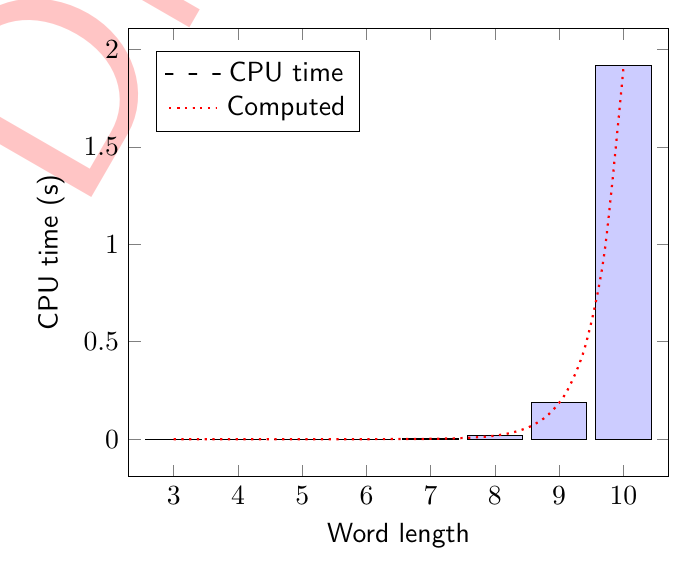
\begin{tikzpicture}
        \begin{axis}[
            xlabel=Word length,
            ylabel=CPU time (s),
            xtick=data, % Afficher une marque pour chaque donnée x
            legend style={at={(0.05,0.95)},anchor=north west}
            ]
        \addplot[ybar, bar width=20pt, fill=blue!20]
            coordinates {
                (3, 5.6425730387369794e-06)
                (4, 1.9073486328125e-05)
                (5, 8.714900297277113e-05)
                (6, 0.0004047552744547526)
                (7, 0.0025780797004699707)
                (8, 0.02060066952424891)
                (9, 0.18696789308027786)
                (10, 1.9171473185221355)
                };
        \addplot[domain=3:10, red, thick, smooth, dotted] {1.52e-10*exp(2.325*x)};
        \legend{CPU time, Computed} 
        \end{axis}
    \end{tikzpicture}
    \caption{Performances testing through process}
\end{figure}


\subsection{Automatic mode}
\subsubsection{Performances}
\subsubsection{Improvements}


\section{Appendices}
\subsection{Personal feedback from this exercise}
\subsection{Interfacing \textit{tikz} and programs}
\subsubsection{Produce dynamic tries with tikz}

\subsubsection{Draw class sumaries}
Plutot que de copier-coller et faire évoluer des morceaux de code séparément pour effectuer les mêmes tâches \textit{tikz}, j'ai choisi de construire une fonction python qui me permet de générer des résumés de chacune des classes utilisées dans les programmes. Cela permet donc de générer de nouveau toutes les illustrations du rapport si un fait évoluer un nom de variable ou qu'on les modifie. D'autre part, cela uniformise le rapport en pouvant changer les couleurs de tous les éléments d'un seul coup.





\end{document}






\begin{figure}[h]
    \centering
    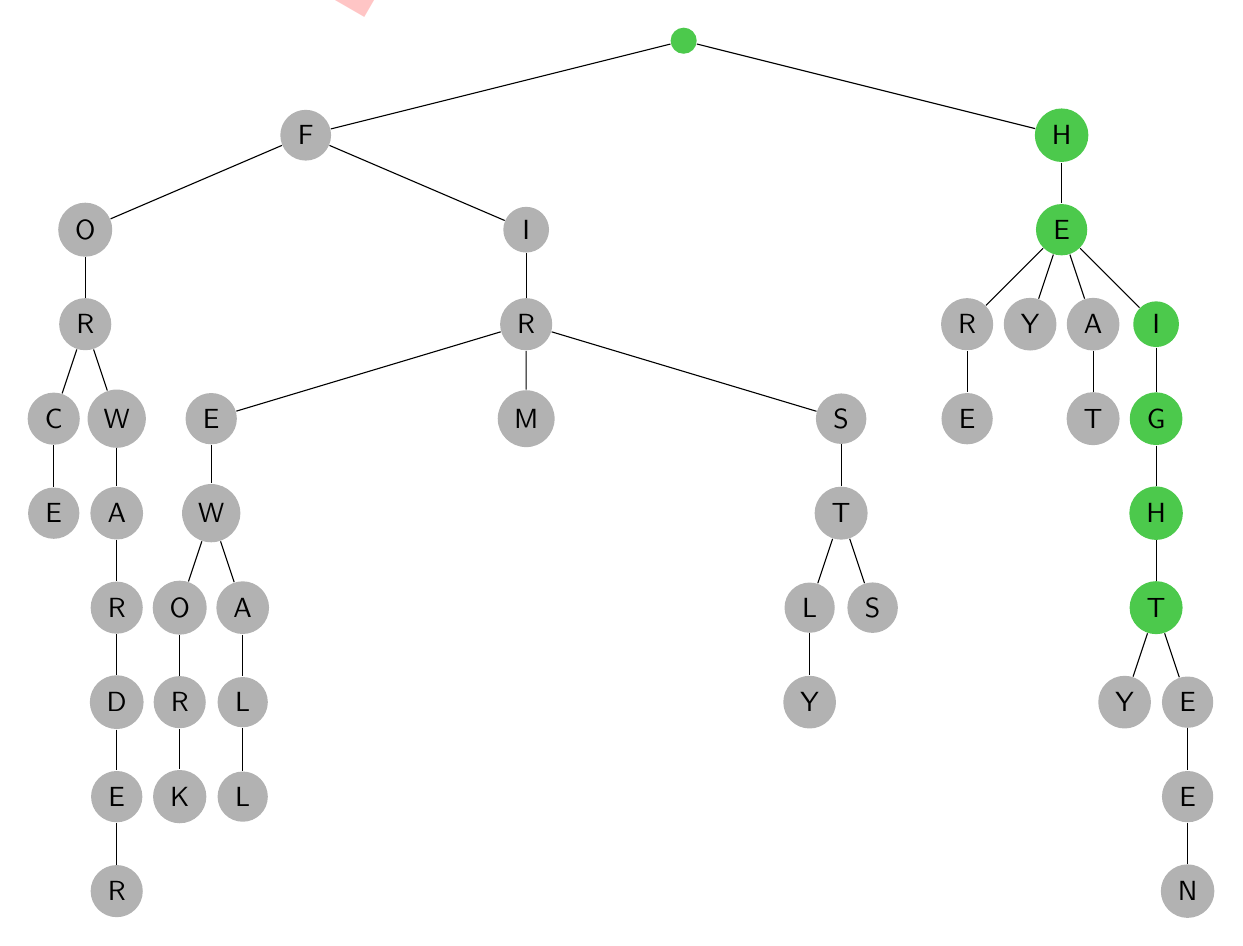
\begin{tikzpicture}[scale=0.8]
\node [circle, fill=green!70!black!70]{}[sibling distance=12cm]
	child{node[circle, fill=black!30]{F}[sibling distance=7cm]
		child{node[circle, fill=black!30]{O}[sibling distance=1cm]
			child{node[circle, fill=black!30]{R}[sibling distance=1cm]
				child{node[circle, fill=black!30]{C}[sibling distance=1cm]
					child{node[circle, fill=black!30]{E}[sibling distance=1cm]
					}
				}
				child{node[circle, fill=black!30]{W}[sibling distance=1cm]
					child{node[circle, fill=black!30]{A}[sibling distance=1cm]
						child{node[circle, fill=black!30]{R}[sibling distance=1cm]
							child{node[circle, fill=black!30]{D}[sibling distance=1cm]
								child{node[circle, fill=black!30]{E}[sibling distance=1cm]
									child{node[circle, fill=black!30]{R}[sibling distance=1cm]
									}
								}
							}
						}
					}
				}
			}
		}
		child{node[circle, fill=black!30]{I}[sibling distance=1cm]
			child{node[circle, fill=black!30]{R}[sibling distance=5cm]
				child{node[circle, fill=black!30]{E}[sibling distance=1cm]
					child{node[circle, fill=black!30]{W}[sibling distance=1cm]
						child{node[circle, fill=black!30]{O}[sibling distance=1cm]
							child{node[circle, fill=black!30]{R}[sibling distance=1cm]
								child{node[circle, fill=black!30]{K}[sibling distance=1cm]
								}
							}
						}
						child{node[circle, fill=black!30]{A}[sibling distance=1cm]
							child{node[circle, fill=black!30]{L}[sibling distance=1cm]
								child{node[circle, fill=black!30]{L}[sibling distance=1cm]
								}
							}
						}
					}
				}
				child{node[circle, fill=black!30]{M}[sibling distance=1cm]
				}
				child{node[circle, fill=black!30]{S}[sibling distance=1cm]
					child{node[circle, fill=black!30]{T}[sibling distance=1cm]
						child{node[circle, fill=black!30]{L}[sibling distance=1cm]
							child{node[circle, fill=black!30]{Y}[sibling distance=1cm]
							}
						}
						child{node[circle, fill=black!30]{S}[sibling distance=1cm]
						}
					}
				}
			}
		}
	}
	child{node[circle, fill=green!70!black!70]{H}[sibling distance=1cm]
		child{node[circle, fill=green!70!black!70]{E}[sibling distance=1cm]
			child{node[circle, fill=black!30]{R}[sibling distance=1cm]
				child{node[circle, fill=black!30]{E}[sibling distance=1cm]
				}
			}
			child{node[circle, fill=black!30]{Y}[sibling distance=1cm]
			}
			child{node[circle, fill=black!30]{A}[sibling distance=1cm]
				child{node[circle, fill=black!30]{T}[sibling distance=1cm]
				}
			}
			child{node[circle, fill=green!70!black!70]{I}[sibling distance=1cm]
				child{node[circle, fill=green!70!black!70]{G}[sibling distance=1cm]
					child{node[circle, fill=green!70!black!70]{H}[sibling distance=1cm]
						child{node[circle, fill=green!70!black!70]{T}[sibling distance=1cm]
							child{node[circle, fill=black!30]{Y}[sibling distance=1cm]
							}
							child{node[circle, fill=black!30]{E}[sibling distance=1cm]
								child{node[circle, fill=black!30]{E}[sibling distance=1cm]
									child{node[circle, fill=black!30]{N}[sibling distance=1cm]
									}
								}
							}
						}
					}
				}
			}
		}
	}
;
\end{tikzpicture}


    \caption{Search path}
    \label{fig:search_path_pgm}
\end{figure}

\begin{figure}[h]
    \centering
    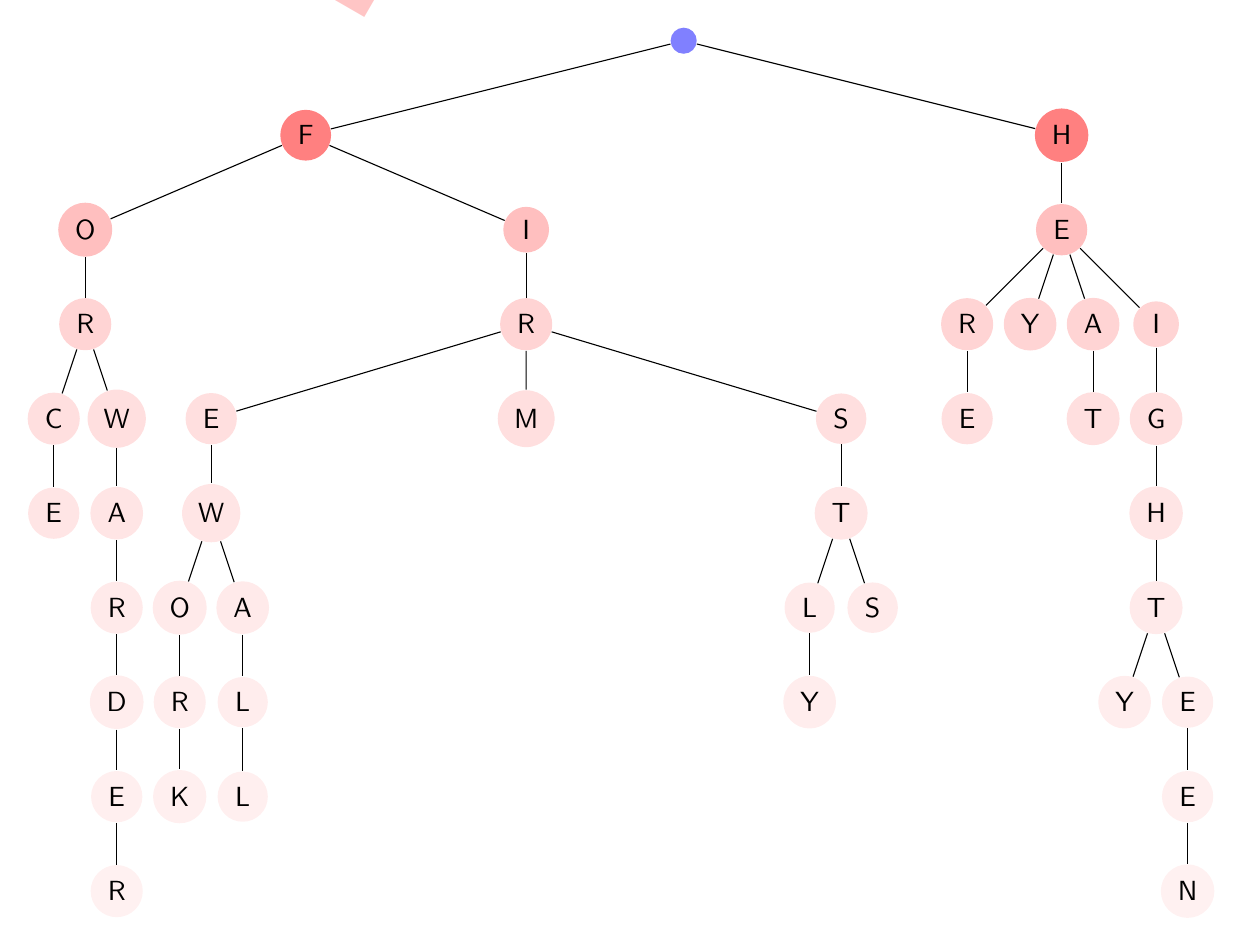
\begin{tikzpicture}[scale=0.8]
\node [circle, fill=blue!50]{}[sibling distance=12cm]
	child{node[circle, fill=red!50.000000]{F}[sibling distance=7cm]
		child{node[circle, fill=red!25.000000]{O}[sibling distance=1cm]
			child{node[circle, fill=red!16.666667]{R}[sibling distance=1cm]
				child{node[circle, fill=red!12.500000]{C}[sibling distance=1cm]
					child{node[circle, fill=red!10.000000]{E}[sibling distance=1cm]
					}
				}
				child{node[circle, fill=red!12.500000]{W}[sibling distance=1cm]
					child{node[circle, fill=red!10.000000]{A}[sibling distance=1cm]
						child{node[circle, fill=red!8.333333]{R}[sibling distance=1cm]
							child{node[circle, fill=red!7.142857]{D}[sibling distance=1cm]
								child{node[circle, fill=red!6.250000]{E}[sibling distance=1cm]
									child{node[circle, fill=red!5.555556]{R}[sibling distance=1cm]
									}
								}
							}
						}
					}
				}
			}
		}
		child{node[circle, fill=red!25.000000]{I}[sibling distance=1cm]
			child{node[circle, fill=red!16.666667]{R}[sibling distance=5cm]
				child{node[circle, fill=red!12.500000]{E}[sibling distance=1cm]
					child{node[circle, fill=red!10.000000]{W}[sibling distance=1cm]
						child{node[circle, fill=red!8.333333]{O}[sibling distance=1cm]
							child{node[circle, fill=red!7.142857]{R}[sibling distance=1cm]
								child{node[circle, fill=red!6.250000]{K}[sibling distance=1cm]
								}
							}
						}
						child{node[circle, fill=red!8.333333]{A}[sibling distance=1cm]
							child{node[circle, fill=red!7.142857]{L}[sibling distance=1cm]
								child{node[circle, fill=red!6.250000]{L}[sibling distance=1cm]
								}
							}
						}
					}
				}
				child{node[circle, fill=red!12.500000]{M}[sibling distance=1cm]
				}
				child{node[circle, fill=red!12.500000]{S}[sibling distance=1cm]
					child{node[circle, fill=red!10.000000]{T}[sibling distance=1cm]
						child{node[circle, fill=red!8.333333]{L}[sibling distance=1cm]
							child{node[circle, fill=red!7.142857]{Y}[sibling distance=1cm]
							}
						}
						child{node[circle, fill=red!8.333333]{S}[sibling distance=1cm]
						}
					}
				}
			}
		}
	}
	child{node[circle, fill=red!50.000000]{H}[sibling distance=1cm]
		child{node[circle, fill=red!25.000000]{E}[sibling distance=1cm]
			child{node[circle, fill=red!16.666667]{R}[sibling distance=1cm]
				child{node[circle, fill=red!12.500000]{E}[sibling distance=1cm]
				}
			}
			child{node[circle, fill=red!16.666667]{Y}[sibling distance=1cm]
			}
			child{node[circle, fill=red!16.666667]{A}[sibling distance=1cm]
				child{node[circle, fill=red!12.500000]{T}[sibling distance=1cm]
				}
			}
			child{node[circle, fill=red!16.666667]{I}[sibling distance=1cm]
				child{node[circle, fill=red!12.500000]{G}[sibling distance=1cm]
					child{node[circle, fill=red!10.000000]{H}[sibling distance=1cm]
						child{node[circle, fill=red!8.333333]{T}[sibling distance=1cm]
							child{node[circle, fill=red!7.142857]{Y}[sibling distance=1cm]
							}
							child{node[circle, fill=red!7.142857]{E}[sibling distance=1cm]
								child{node[circle, fill=red!6.250000]{E}[sibling distance=1cm]
									child{node[circle, fill=red!5.555556]{N}[sibling distance=1cm]
									}
								}
							}
						}
					}
				}
			}
		}
	}
;
\end{tikzpicture}


    \caption{Draw trie}
    \label{fig:draw_pgm}
\end{figure}



\section{Data structure}
\subsection{Tries implementation}


\section{Performances}
\begin{summary}
    Essai
\end{summary}


\section{Complexity and time preduction}


\begin{figure}
    \centering
    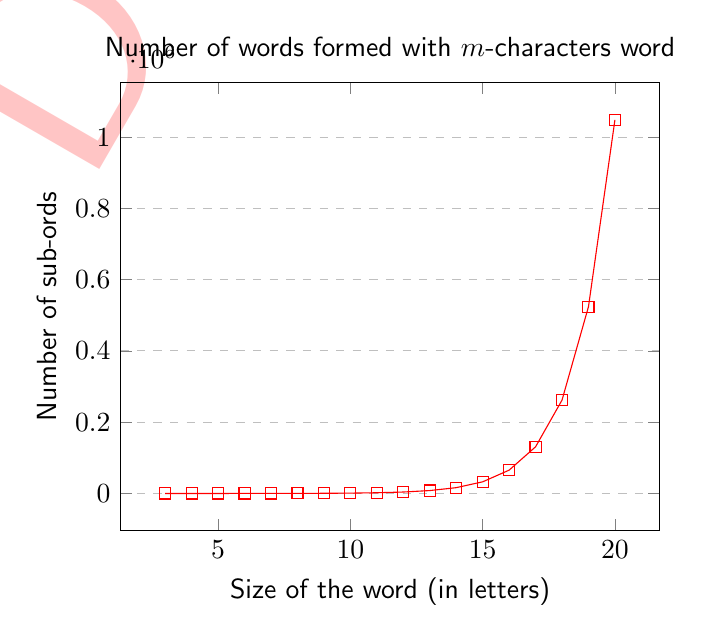
\begin{tikzpicture}
\begin{axis}[
    title={Number of words formed with $m$-characters word},
    xlabel={Size of the word (in letters)},
    ylabel={Number of sub-ords},
    % xmin=0, xmax=100,
    % ymin=0, ymax=120,
    % xtick={0,20,40,60,80,100},
    % ytick={0,20,40,60,80,100,120},
    legend pos=north west,
    ymajorgrids=true,
    grid style=dashed,
]

\addplot[
    color=red,
    mark=square,
    ]
    coordinates {
        (3, 0)
        (4, 4)
        (5, 15)
        (6, 41)
        (7, 98)
        (8, 218)
        (9, 465)
        (10, 967)
        (11, 1980)
        (12, 4016)
        (13, 8099)
        (14, 16277)
        (15, 32646)
        (16, 65398)
        (17, 130917)
        (18, 261971)
        (19, 524096)
        (20, 1048364)
    };
    
\end{axis}
\end{tikzpicture}

    \caption{A PGF histogram from \texttt{matplotlib}.}
\end{figure}

As a consequence, we have to find a way to decrease the number of 

\section{Ideas}
Change the programmation philosophy to:
\begin{itemize}
    \item Définition des fonctions de jeu par récurrence: appel de la fonction avec comme paramètres
        \begin{itemize}
            \item Mot à deviner (secret)
            \item Mot choisi par l'utilisateur
            \item Résultat (en terme de 0, 1, 2)
            \item Numéro de l'essais 
        \end{itemize}
        Cela permettra de faire appel aux fonctions par récurrence et de mutualiser les programmes de \textit{guesser} et de \textit{keeper}
    \item Passer en programmation par objet avec un objet pour :
        \begin{itemize}
            \item guesser
            \item keeper
            \item guess
            \item secret
            \item tentative
        \end{itemize}
\end{itemize}

\section{Best practices}
\begin{itemize}
    \item Description des fonctions avec docstring
    \item Ajout des typages pour les fonctions (aide à l'IDE)
    \item Mise en commun des fonctions identiques (factorisation)
    \item Tentative d'optimisation
\end{itemize}



\section{Objects}
\begin{figure}[h]
    \centering
    \begin{tikzpicture}
        \node[draw, rounded corners=2mm, inner sep = 0.2cm, fill=orange!0] { 
        \begin{tikzpicture} 
            \node[inner sep = 1mm] (title) { \Large{\bfseries Guess }}; 
            % \draw (title.south west) -- (title.south east);
            \node[at=(title.south), anchor=north, inner sep=3mm, align=left, fill=green!30!black!10, yshift=-0.2cm] (attributes) {
                \begin{minipage}{60mm}
                    \textbf{Attributes}\\
                    \small{0}: \verb|letters|\\
\small{1}: \verb|length|\\
\small{2}: \verb|alphabet|\\
\small{3}: \verb|incorrect_position_letters|\\
\small{4}: \verb|bad_letters|\\
\small{5}: \verb|remaining_letters|\\
\small{6}: \verb|dictionary_trie|
                \end{minipage} 
                };
            % \draw (attributes.north west) -- (attributes.north east);
            \node[at=(attributes.south), anchor=north, inner sep=3mm, align=left, fill=blue!10, yshift=-0.2cm] (methods) {
                \begin{minipage}{60mm}
                    \textbf{Methods}\\
                    \small{0}: \verb|actualize_letter|\\
\small{1}: \verb|actualize_letters_informations|\\
\small{2}: \verb|display_word|\\
\small{3}: \verb|extract_random_letter|\\
\small{4}: \verb|generate_new_letters|\\
\small{5}: \verb|is_valid_word|\\
\small{6}: \verb|new_guess|
                \end{minipage} 
                };
            % \draw (methods.north west) -- (methods.north east);
        \end{tikzpicture}
        }; 
    \end{tikzpicture}
    \caption{Class description - Guess }
    \label{class:Guess}
\end{figure}
\begin{figure}[h]
    \centering
    \begin{tikzpicture}
        \node[draw, rounded corners=2mm, inner sep = 0.2cm, fill=orange!0] { 
        \begin{tikzpicture} 
            \node[inner sep = 1mm] (title) { \Large{\bfseries Trie }}; 
            % \draw (title.south west) -- (title.south east);
            \node[at=(title.south), anchor=north, inner sep=3mm, align=left, fill=green!30!black!10, yshift=-0.2cm] (attributes) {
                \begin{minipage}{60mm}
                    \textbf{Attributes}\\
                    \small{0}: \verb|root|
                \end{minipage} 
                };
            % \draw (attributes.north west) -- (attributes.north east);
            \node[at=(attributes.south), anchor=north, inner sep=3mm, align=left, fill=blue!10, yshift=-0.2cm] (methods) {
                \begin{minipage}{60mm}
                    \textbf{Methods}\\
                    \small{0}: \verb|insert_word|\\
\small{1}: \verb|search|\\
\small{2}: \verb|word_game_main_function|
                \end{minipage} 
                };
            % \draw (methods.north west) -- (methods.north east);
        \end{tikzpicture}
        }; 
    \end{tikzpicture}
    \caption{Class description - Trie }
    \label{class:Trie}
\end{figure}
\begin{figure}[h]
    \centering
    \begin{tikzpicture}
        \node[draw, rounded corners=2mm, inner sep = 0.2cm, fill=orange!0] { 
        \begin{tikzpicture} 
            \node[inner sep = 1mm] (title) { \Large{\bfseries TrieNode }}; 
            % \draw (title.south west) -- (title.south east);
            \node[at=(title.south), anchor=north, inner sep=3mm, align=left, fill=green!30!black!10, yshift=-0.2cm] (attributes) {
                \begin{minipage}{60mm}
                    \textbf{Attributes}\\
                    \small{0}: \verb|children|\\
\small{1}: \verb|is_end_word|\\
\small{2}: \verb|value|\\
\small{3}: \verb|depth|
                \end{minipage} 
                };
            % \draw (attributes.north west) -- (attributes.north east);
            \node[at=(attributes.south), anchor=north, inner sep=3mm, align=left, fill=blue!10, yshift=-0.2cm] (methods) {
                \begin{minipage}{60mm}
                    \textbf{Methods}\\
                    \small{0}: \verb|leaves_counter_recursive|
                \end{minipage} 
                };
            % \draw (methods.north west) -- (methods.north east);
        \end{tikzpicture}
        }; 
    \end{tikzpicture}
    \caption{Class description - TrieNode }
    \label{class:TrieNode}
\end{figure}
\begin{figure}[h]
    \centering
    \begin{tikzpicture}
        \node[draw, rounded corners=2mm, inner sep = 0.2cm, fill=orange!0] { 
        \begin{tikzpicture} 
            \node[inner sep = 1mm] (title) { \Large{\bfseries WordLetter }}; 
            % \draw (title.south west) -- (title.south east);
            \node[at=(title.south), anchor=north, inner sep=3mm, align=left, fill=green!30!black!10, yshift=-0.2cm] (attributes) {
                \begin{minipage}{60mm}
                    \textbf{Attributes}\\
                    \small{0}: \verb|index|\\
\small{1}: \verb|past_letters|\\
\small{2}: \verb|score|\\
\small{3}: \verb|blocked_letter|\\
\small{4}: \verb|current_letter|
                \end{minipage} 
                };
            % \draw (attributes.north west) -- (attributes.north east);
            \node[at=(attributes.south), anchor=north, inner sep=3mm, align=left, fill=blue!10, yshift=-0.2cm] (methods) {
                \begin{minipage}{60mm}
                    \textbf{Methods}\\
                    \small{0}: \verb|add_letter_guess|\\
\small{1}: \verb|add_past_letter|\\
\small{2}: \verb|block_letter|\\
\small{3}: \verb|is_past_letter|\\
\small{4}: \verb|update_score|
                \end{minipage} 
                };
            % \draw (methods.north west) -- (methods.north east);
        \end{tikzpicture}
        }; 
    \end{tikzpicture}
    \caption{Class description - WordLetter }
    \label{class:WordLetter}
\end{figure}

\end{document}
